% this file is called up by thesis.tex
% content in this file will be fed into the main document

\chapter{Evaluation}\label{ch:evaluation} % top level followed by section, subsection


% ----------------------- paths to graphics ------------------------

% change according to folder and file names
\ifpdf
    \graphicspath{{figures/PNG}}
\else
    \graphicspath{{7/figures/EPS/}{7/figures/}}
\fi


% ----------------------- contents from here ------------------------
% 
In this section, the experimental results are presented.
The RDMA transportation types are compared within and against the baseline TCP implementation.
Throughput and latency are mainly used to analysis the multicore scalability of these transportation types, with increasing number of clients, and therefore threads.
For latency three figures have been used to evaluate: average latency, boxplot without outliers, and cumulative distribution function (CDF).
The same raw data is used for both measurements, thus can be compared alongside each other.
The two designs are analyzed, with and without waiting for completion event.

In short, the results show:
\begin{itemize}
    \item Without blocking, throughput reaches an peak, with all transportation types, at roughly 32 clients.
    UC performs best, with a maximum throughput of 370185 ops/sec at 33 clients.
    Further details are given in section \ref{sec:throughput-analysis}.
    \item With blocking, throughput reaches an equilibrium up to 70 clients, on all types: TCP, RC and UC.
    UC, again, performance best, stabilizing at roughly 272717 ops/sec above 32 clients.
    \item Latency increases across all transportation types, with increased number of clients, and both with and without blocking.
    Results are inversely comparable to throughput, again with UC performing best.
    Without blocking: UC has an average latency of roughly 49.2 $\mu$sec at 32 clients and 179.7 $\mu$sec at 60 clients.
    The spread also increases: standard deviation ranges from 46.6 $\mu$sec at 32 clients, to 1628.2 $\mu$sec at 60 clients.
    UC also performance best due to the stable 95th percentile, which is 110 $\mu$sec for both 32 and 60 clients.

    With blocking: UC has a average latency of roughly 99.3 $\mu$sec at 32 clients and 158.3 $\mu$sec at 60 clients, and scales in a linear relation.
    The spread also increases: standard deviation ranges from 150.7 $\mu$sec at 32 clients, to 326.8 $\mu$sec at 60 clients.

    Section \ref{sec:latency:analysis} delves deeper with statistical analysis.
\end{itemize}

To recall the benchmarking setup:
Ten million KV-store operations are divided equally between \textit{n}-clients.

\section{Throughput analysis}\label{sec:throughput-analysis}
To compare the overall throughput between TCP, RC, UC, and UD with up to 70 clients.
Both designs, with and without waiting for completion event, are analyzed.

\subsection{Throughput analysis without waiting for completion event}
With non-blocking design, peak throughput performance is realised at roughly 32 clients.
This can be seen in figure \ref{fig:throughput-70}.
For RC, maximum throughput is roughly 247782 ops/sec at 32 clients.
While for UC, maximum throughput is roughly 370185 ops/sec at 33 clients, and for UD this is at roughly 357019 ops/sec at 31 clients.
The maximum throughput TCP achieves in this number of clients range, is 206750 ops/sec at 33 clients.
For RC, UC, and UD this is a percentage increase over TCP of: 19.85\%, 79.05\%, and 72.68\%.
However, after 32 clients, throughput has a sharp decline, with RC failing to connect properly above 60 clients, resulting in incomplete data at these points.
\begin{figure}
    \centering
    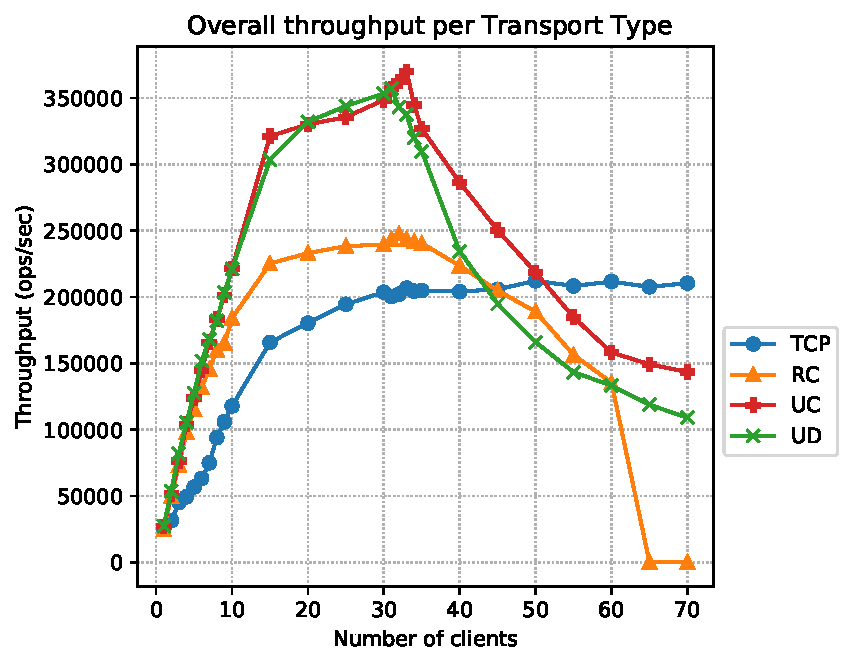
\includegraphics[height=8cm]{figures/PDF/Throughput_70}
    \caption[Throughput of clients executing 10 million key-value operations.]{Throughput of clients executing 10 million key-value operations. Note: RC could not connect reliably above 60 clients, thus removed.}
    \label{fig:throughput-70}
\end{figure}

\subsubsection{Scalability rate}\label{subsec:scalability-rate}
Multicore scalability of all RDMA transportation types, without blocking, is poor.
Up to roughly 15 clients, throughput performance increases at a linear rate.
For TCP, there is an average increase of 10246 ops/sec per additional client.
For the RDMA transport types, for RC this is 16726 ops/sec per additional client, 21462 ops/sec for UC, and 21067 ops/sec for UD.
This shows that unreliable transport types, UC and UD, scale better per additional client and worker thread, compared to RC and TCP.
However, after 15 threads, performance begins to plateau for all transportation types and TCP, showing that the used KV-store is CPU bound.
This is due to the pthread locking, used to provide isolation with concurrent threads operating on the KV-store.

After 32 clients and worker threads, multicore performance weakens, and dropping in performance.
This is due to the non-blocked design, and 32 physical threads being the maximum on a single DAS-5 node.
Without this blocking or scheduling, threads take CPU cycles while polling on the receive queue.
With only a limited number of CPU cycles, this is not used efficiently, resulting in drop in performance for all worker threads.

\begin{table}
    \centering
    \begin{tabular}{rllll}
        \toprule
        \textbf{Clients} & \textbf{TCP} & \textbf{RC} & \textbf{UC} & \textbf{UD} \\
        \midrule
        1 &  &  &  &  \\
        2 & 6531.57 & 24686.53 & 24638.92 & 26502.61 \\
        3 & 13594.19 & 23770.88 & 24785.06 & 28301.23 \\
        4 & 4297.08 & 24568.10 & 27795.82 & 23489.22 \\
        5 & 7363.60 & 17665.62 & 19850.78 & 22090.11 \\
        6 & 6521.77 & 16064.32 & 20579.03 & 24167.81 \\
        7 & 11672.15 & 13975.28 & 21439.07 & 16246.35 \\
        8 & 18989.11 & 14401.89 & 17510.51 & 14201.32 \\
        9 & 12033.20 & 4957.15 & 17930.69 & 21432.35 \\
        10 & 11858.04 & 18916.31 & 20129.91 & 17827.71 \\
        15 & 9603.18 & 8252.11 & 19962.03 & 16410.47 \\
        \bottomrule
    \end{tabular}
    \caption[Change in throughput per additional client, up to 15 clients.]{Change in throughput per additional client, up to 15 clients. Values are shown in ops/sec per additional client.}
    \label{tab:throughput_add_client}
\end{table}

\subsection{Throughput analysis by waiting for completion event}




\section{Latency analysis}\label{sec:latency:analysis}
An important factor to KV-store is their quick response time.
Latency should ideally scale similarly, preferably better, than throughput, such that with an increased number of clients, latency changes are unnoticed to clients.
RDMA should offer faster response time, by their bypassing kernel design.
In this section, the extent of this is explored, for both methods of polling: with and without waiting for completion event by blocking.

\subsection{Latency analysis without waiting for completion event}

\begin{figure}
    \centering
    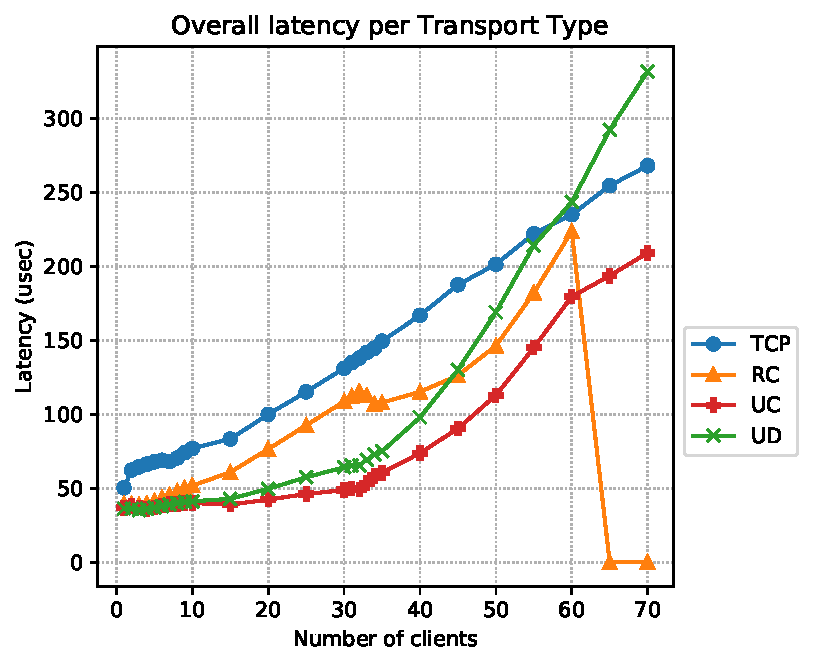
\includegraphics[width=\columnwidth]{figures/PDF/Latency_avg_70}
    \caption{Latency of clients executing 10 million key-value operations}
    \label{fig:latency-70}
\end{figure}

With a polling, non-blocking design, RDMA transportation types perform better than TCP up to 55 clients, after which UD performs worse, and RC following this trend. This can be seen in \ref{fig:latency-70}.
At roughly 32 clients, ranking is similar to throughput as seen in figure \ref{fig:throughput-70}.
Results show that TCP has an average latency of 138.0 $\mu$sec at 32 clients.
RC has an average latency of 115.1 $\mu$sec, a 16.61\% improvement relative to TCP.
UC performs best at 32 clients, with an average latency of 49.24 $\mu$sec, which is an 64.33\% improvement over TCP.
Finally, UD has an average latency of 65.5 $\mu$sec, which is an improvement of 52.5\% over TCP.

It can also be observed that latency scales proportional with the number of clients for TCP, while this is only the case for RDMA transport types up to roughly 32 clients.
The average rate of change for TCP, RC, UC, and UD up to 32 clients is: 2.31 $\mu$sec, 2.00 $\mu$sec, 0.37 $\mu$sec, and 0.72 $\mu$sec.
This shows that UC scales favorably up to 32 clients, closely followed by UD.
After 32 clients, RDMA transport types scale worse, with UD surpassing TCP's average latency at 60 clients.
RC is trending towards surpassing TCP after 60 clients, however, this data could not be collected reliably.
Lastly, UC still performs favorably compared to TCP at 70 clients, however, relative performance is now at 21.98\%.

\subsubsection{Variation in Latency performance}
Consistent latency is important for clients, such that performance is predictable, and provide reliable services to end users.
To examine the variation in latency with increasing number of clients visually, two types of graphs are used: box plot and CDF graph.
Graphs show the spread in latency results at three points: 5 clients, 32 clients and 60 clients.
Additionally, the median, innerquartile range, 95th and 99th percentile, and standard deviation, is used to examine the spread numerically.
This numeric data can be found in table \ref{tab:num_stats}, for the three sets of data.
A complete table, with all number of clients up to 70, can be found in table INSERT TABLE in the appendix.
\begin{table}
    \subtable[TCP] {
        \centering
        \begin{tabular}{rrrrrr}
            \toprule
            \textbf{Clients} & \textbf{Median} & \textbf{IQR} & \textbf{95th percentile} & \textbf{99th percentile} & \textbf{Standard deviation} \\
            \midrule
            5 & 62 & 55 & 126 & 152 & 33.50 \\
            32 & 129 & 40 & 192 & 233 & 268.86 \\
            60 & 238 & 65 & 318 & 368 & 275.85 \\
            \bottomrule
        \end{tabular}
        \label{tab:num_stats_tcp}
    }

    \subtable[RC] {
        \centering
        \begin{tabular}{rrrrrr}
            \toprule
            \textbf{Clients} & \textbf{Median} & \textbf{IQR} & \textbf{95th percentile} & \textbf{99th percentile} & \textbf{Standard deviation} \\
            \midrule
            5 & 31 & 43 & 88 & 99 & 29.33 \\
            32 & 112 & 149 & 227 & 231 & 83.10 \\
            60 & 48 & 56 & 120 & 7852.41 & 1662.83 \\
            \bottomrule
        \end{tabular}
        \label{tab:num_stats_rc}
    }

    \subtable[UC] {
        \centering
        \begin{tabular}{rrrrrr}
            \toprule
            \textbf{Clients} & \textbf{Median} & \textbf{IQR} & \textbf{95th percentile} & \textbf{99th percentile} & \textbf{Standard deviation} \\
            \midrule
            5 & 29 & 49 & 84 & 95 & 29.26 \\
            32 & 39 & 70 & 110 & 122 & 46.59 \\
            60 & 35 & 56 & 110 & 1296 & 1629.16 \\
            \bottomrule
        \end{tabular}
        \label{tab:num_stats_uc}
    }

    \subtable[UD] {
        \centering
        \begin{tabular}{rrrrrr}
            \toprule
            \textbf{Clients} & \textbf{Median} & \textbf{IQR} & \textbf{95th percentile} & \textbf{99th percentile} & \textbf{Standard deviation} \\
            \midrule
            5 & 29 & 46 & 84 & 95 & 30.45 \\
            32 & 57 & 64 & 126 & 146 & 65.59 \\
            60 & 54 & 65 & 143 & 9036 & 1693.72 \\
            \bottomrule
        \end{tabular}
        \label{tab:num_stats_ud}
    }

    \caption{Numeric statistic latency. All statistical values have unit $\mu$sec. IRQ is short for innerquartile range}
    \label{tab:num_stats}
\end{table}

\begin{figure}
    \centering
    \subfigure[5 clients] {
        \centering
        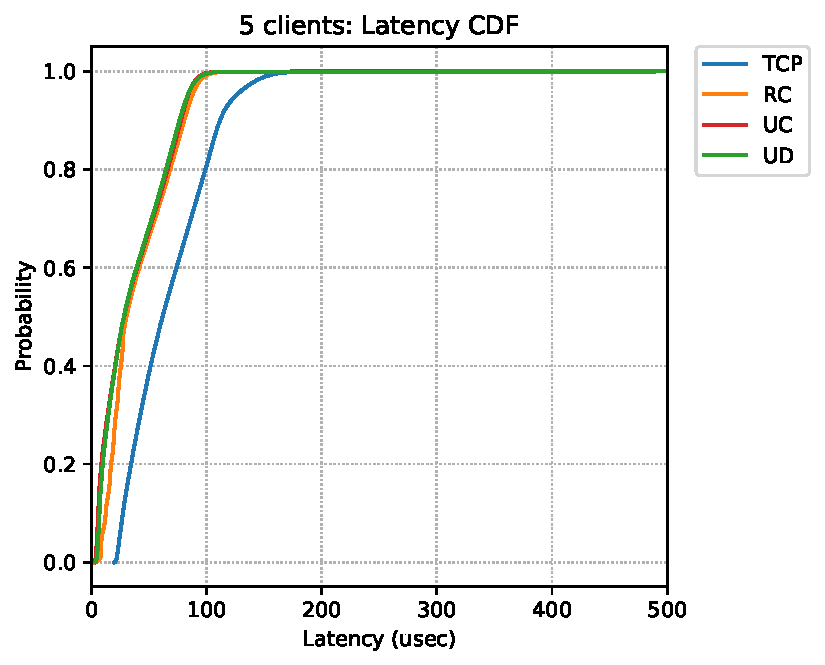
\includegraphics[width=0.47\columnwidth]{figures/PDF/Latency_cdf_5}
        \label{fig:cdf_5}
    }
    \subfigure[32 clients] {
        \centering
        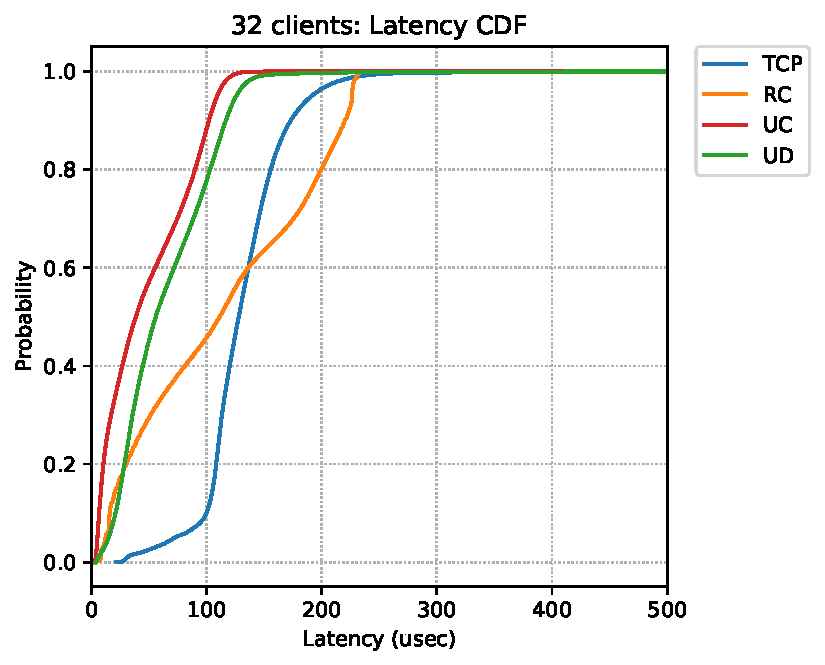
\includegraphics[width=0.47\columnwidth]{figures/PDF/Latency_cdf_32}
        \label{fig:cdf_32}
    }
    \subfigure[60 clients] {
        \centering
        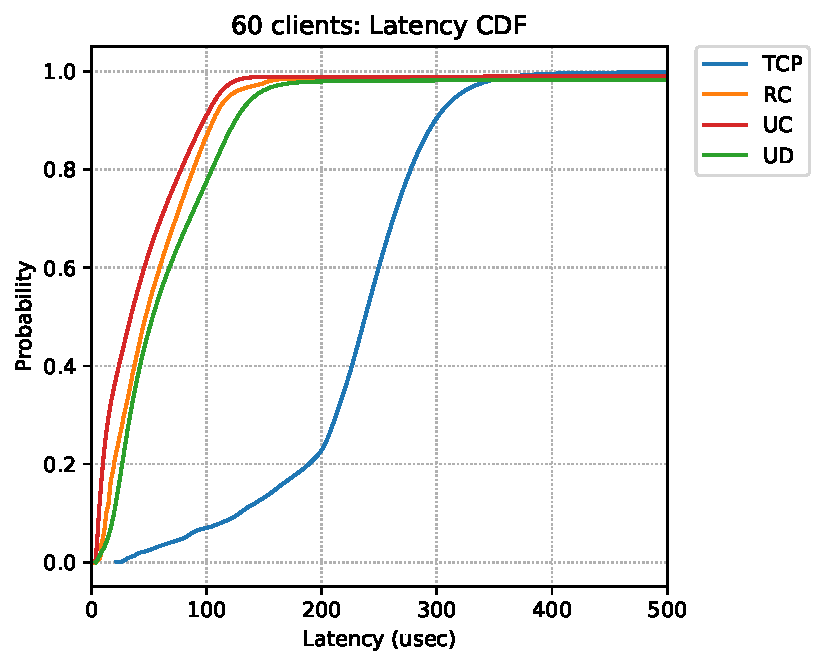
\includegraphics[width=0.47\columnwidth]{figures/PDF/Latency_cdf_60}
        \label{fig:cdf_60}
    }
    \caption[Latency cumulative distribution function (CDF)]{Latency cumulative distribution function (CDF) for 5, 32 and 60 clients. }
    \label{fig:CDF}
\end{figure}


\begin{figure}
    \centering
    \subfigure[5 clients] {
        \centering
        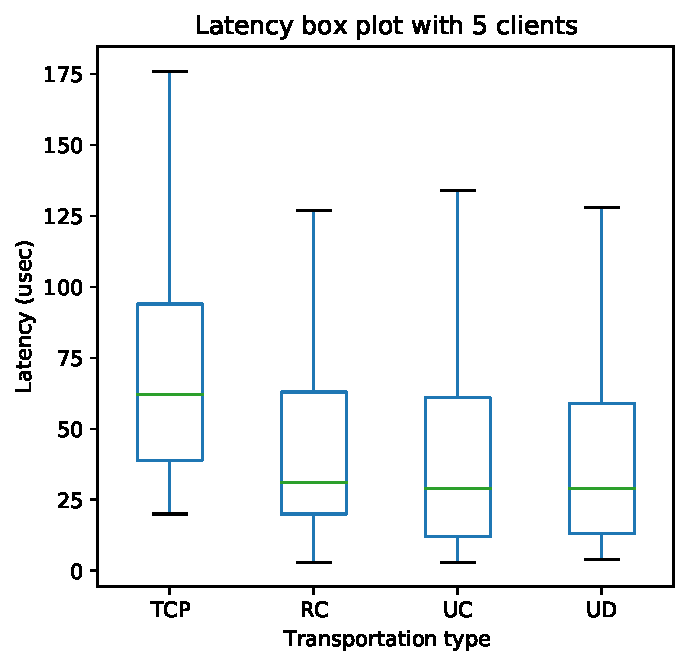
\includegraphics[width=0.47\columnwidth]{figures/PDF/Latency_box_no_out_5}
        \label{fig:box_5}
    }
    \subfigure[32 clients] {
        \centering
        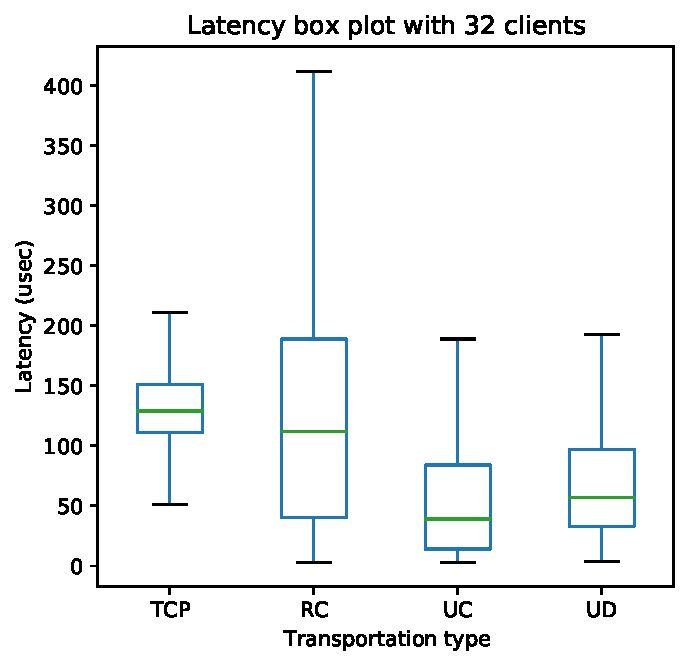
\includegraphics[width=0.47\columnwidth]{figures/PDF/Latency_box_no_out_32}
        \label{fig:box_32}
    }
    \subfigure[60 clients] {
        \centering
        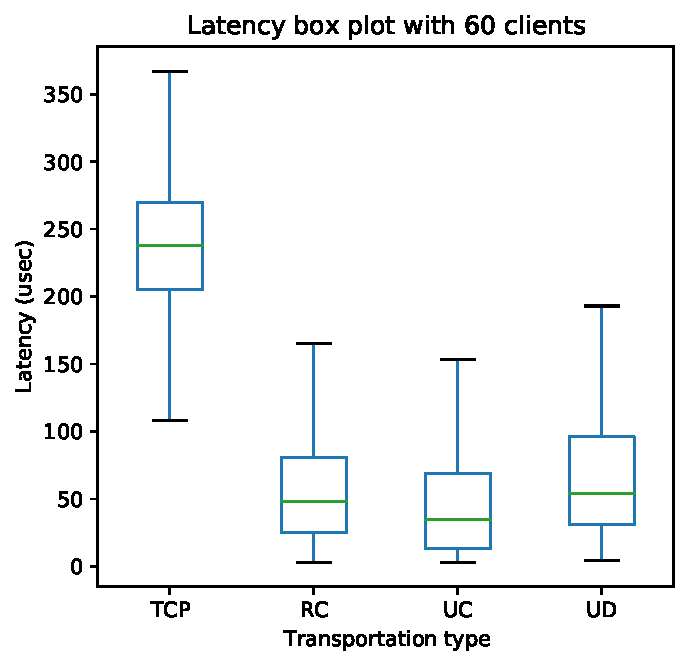
\includegraphics[width=0.47\columnwidth]{figures/PDF/Latency_box_no_out_60}
        \label{fig:box_60}
    }
    \caption[Latency box plot]{Latency box plot for 5, 32 and 60 clients. }
    \label{fig:Box}
\end{figure}

From table \ref{tab:num_stats} it can be observed that for 5, 32 and 60 clients, standard deviation increases as number of clients increase.
With RDMA, there is a significant increase in variation after 32 clients.
The median latency and 95th percentile of UC and UD remains similiar between 32 and 60 clients, however the outliers or 99th percentile, increase significantly, this can be seen in \ref{tab:num_stats}.
This is further supported by the CDF figure of 32 clients, figure \ref{fig:cdf_32}, and 60 clients, \ref{fig:cdf_60}.
In these figures, 80\% of the data is near 100 $\mu$sec and 90 $\mu$sec, for UD and UC respectively, deviating slightly between 32 and 60 clients.
However, the top 1\% of the data is not below the 500 $\mu$sec shown for 60 clients, while this is the case for 32 clients.
These outliers are caused by polling with concurrent number of threads, which exceed the number of physical threads.
With high CPU usage, the time until a new request is seen and can be processed, increases, causing a delay for the client.
These outliers can be the cause of loss in throughput performance, seen in figure \ref{fig:throughput-70}.

It can also be observed that RC suffers from a peak spread around 32 clients, which afterwards declines.
This can be seen in table \ref{tab:num_stats_rc} and figure \ref{fig:Box}.
Innerquartile range reaches a peak of 149 $\mu$sec at 32 clients, at a median of 112 $\mu$sec.
It is unclear what causes this, however should be considered when reaching maximum number of physical threads.

\subsection{Latency analysis by waiting for completion event}


% ---------------------------------------------------------------------------
% ----------------------- end of thesis sub-document ------------------------
% ---------------------------------------------------------------------------